%% This is file `elsarticle-template-1a-num.tex',
%%
%% Copyright 2009 Elsevier Ltd
%%
%% This file is part of the 'Elsarticle Bundle'.
%% ---------------------------------------------
%%
%% It may be distributed under the conditions of the LaTeX Project Public
%% License, either version 1.2 of this license or (at your option) any
%% later version.  The latest version of this license is in
%%    http://www.latex-project.org/lppl.txt
%% and version 1.2 or later is part of all distributions of LaTeX
%% version 1999/12/01 or later.
%%
%% The list of all files belonging to the 'Elsarticle Bundle' is
%% given in the file `manifest.txt'.
%%
%% Template article for Elsevier's document class `elsarticle'
%% with numbered style bibliographic references
%%
%% $Id: elsarticle-template-1a-num.tex 151 2009-10-08 05:18:25Z rishi $
%% $URL: http://lenova.river-valley.com/svn/elsbst/trunk/elsarticle-template-1a-num.tex $
%%
\documentclass[preprint,12pt]{elsarticle}

%% Use the option review to obtain double line spacing
%% \documentclass[preprint,review,12pt]{elsarticle}

%% Use the options 1p,twocolumn; 3p; 3p,twocolumn; 5p; or 5p,twocolumn
%% for a journal layout:
%% \documentclass[final,1p,times]{elsarticle}
%% \documentclass[final,1p,times,twocolumn]{elsarticle}
%% \documentclass[final,3p,times]{elsarticle}
%% \documentclass[final,3p,times,twocolumn]{elsarticle}
%% \documentclass[final,5p,times]{elsarticle}
%% \documentclass[final,5p,times,twocolumn]{elsarticle}

%% if you use PostScript figures in your article
%% use the graphics package for simple commands
%% \usepackage{graphics}
%% or use the graphicx package for more complicated commands
%% \usepackage{graphicx}
%% or use the epsfig package if you prefer to use the old commands
%% \usepackage{epsfig}

%% The amssymb package provides various useful mathematical symbols
\usepackage{amssymb}
%% The amsthm package provides extended theorem environments
%% \usepackage{amsthm}

%% The lineno packages adds line numbers. Start line numbering with
%% \begin{linenumbers}, end it with \end{linenumbers}. Or switch it on
%% for the whole article with \linenumbers after \end{frontmatter}.
%% \usepackage{lineno}

%% natbib.sty is loaded by default. However, natbib options can be
%% provided with \biboptions{...} command. Following options are
%% valid:

%%   round  -  round parentheses are used (default)
%%   square -  square brackets are used   [option]
%%   curly  -  curly braces are used      {option}
%%   angle  -  angle brackets are used    <option>
%%   semicolon  -  multiple citations separated by semi-colon
%%   colon  - same as semicolon, an earlier confusion
%%   comma  -  separated by comma
%%   numbers-  selects numerical citations
%%   super  -  numerical citations as superscripts
%%   sort   -  sorts multiple citations according to order in ref. list
%%   sort&compress   -  like sort, but also compresses numerical citations
%%   compress - compresses without sorting
%%
%% \biboptions{comma,round}

% \biboptions{}
\usepackage[utf8]{inputenc}
\usepackage{pseudocode}
\usepackage{pstricks}
\usepackage{amsmath}
\usepackage{amsfonts}   % if you want the fonts
\usepackage{amssymb}    % if you want extra symbols
\usepackage{subfigure}
\usepackage{graphicx}
\usepackage{multirow}
\usepackage{color}
\usepackage[T1]{fontenc}

%% criar Hline mais grossa
\newdimen\arrayruleHwidth
\setlength{\arrayruleHwidth}{2pt}
\makeatletter
\def\Hline{\noalign{\ifnum0=‘}\fi\hrule \@height \arrayruleHwidth
\futurelet \@tempa\@xhline}

\makeatletter
\def\etc{\emph{etc. }} \def\vs{\emph{vs. }}
\def\ie{\emph{i.e. }} \def\Ie{\emph{I.e. }}
\makeatother

\journal{Information Sciences}

\begin{document}

\begin{frontmatter}

%% Title, authors and addresses

%% use the tnoteref command within \title for footnotes;
%% use the tnotetext command for the associated footnote;
%% use the fnref command within \author or \address for footnotes;
%% use the fntext command for the associated footnote;
%% use the corref command within \author for corresponding author footnotes;
%% use the cortext command for the associated footnote;
%% use the ead command for the email address,
%% and the form \ead[url] for the home page:
%%
%% \title{Title\tnoteref{label1}}
%% \tnotetext[label1]{}
%% \author{Name\corref{cor1}\fnref{label2}}
%% \ead{email address}
%% \ead[url]{home page}
%% \fntext[label2]{}
%% \cortext[cor1]{}
%% \address{Address\fnref{label3}}
%% \fntext[label3]{}

\title{Multidimensional Quick Invariant Signature Extraction}

%% use optional labels to link authors explicitly to addresses:
%% \author[label1,label2]{<author name>}
%% \address[label1]{<address>}
%% \address[label2]{<address>}

\author[ualg]{Hamid Reza Shahbazkia} 

\address[ualg]{University of Algarve\\
Department of Electronics and Informatics Engineering\\
8005-139 Faro, Portugal\\
hshah@ualg.pt}

\author[ualg,dtu]{António dos Anjos}

\author[dtu]{Katarzyna G\k{e}bal}

\address[dtu]{DTU Informatics\\
2800 Kgs. Lyngby, Denmark\\
aanjos@imm.dtu.dk, katg@imm.dtu.dk}


\begin{abstract}
%% Text of abstract
Simple geometric properties can be used to define the signature of a pixel pattern independently of its position, size or orientation in an image. These properties can be extended to obtain invariances in volumes or even in any N-dimensional data space.
In this paper we present a simple and fast approach to create a Quick Invariant Signature (QIS), that can be used for usual affine transformations as well as for other transformations such as toric or cylindrical translation or window size modifications.
The signature extraction is performed in data space and directly on points without any estimation or compression. We provide a formal demonstration that the signature is totally invariant in any N-dimensional space, studying the case of 2-D images, before extending the notion to many dimensional spaces.
\end{abstract}

\begin{keyword}
%% keywords here, in the form: keyword \sep keyword
Shape matching \sep invariant descriptor \sep image signature.
%% MSC codes here, in the form: \MSC code \sep code
%% or \MSC[2008] code \sep code (2000 is the default)

\end{keyword}

\end{frontmatter}

%%
%% Start line numbering here if you want
%%
% \linenumbers

%% main text
\section{Introduction}
Data analysis often requires considering the possible transformations the data has been subjected to. In a vision system for example, invariance to translation is a usual and straightforward requirement. Many different approaches to obtain invariance in 2-D images for pattern recognition have been developed and largely used \cite{moments1,moments2,fm1,tm1,omm1}. We can classify them into three main classes: Invariant moments, invariant descriptors, and invariant neural architectures. Invariant moments \cite{moments3} and Fourier-Mellin descriptors \cite{fm2,fm3} require complex calculations and significant computation time. They are quite sensitive to noise and images cannot be directly analyzed. Therefore only a few of the interest points are taken into consideration. Other invariant descriptors, such as the circular descriptor, are highly sensitive to noise and can cause sampling problems.
The most popular neural-network approach \cite{Spirkovska1990,nn1}, a multi-layer perceptron network and a back-propagation learning algorithm, requires a huge training set to learn the invariance to affine 2-D transformations. Other neural networks try to integrate invariance into their architectures but this causes a problem of network size by combinatorial explosion that seriously limits the size of their input.
The Quick Invariant Signature (QIS) extraction proposed here is a formal method which uses simple geometric notions such as length and slope to define the invariant signature of a binary image. The size of the input is not limited and no pre-processing is needed. The only requirement is that the image is binary, for example, the result of an edge detection operation. The whole image is taken into account for the extraction of the signature.
In \cite{Shahbazkia2009} we presented an approach to define a binary image in terms of active couples of points as well as algorithms to extract the signatures.
The multidimensional QIS presented here simplifies and extends these approaches.
QIS can be used to extract a signature, not only invariant to classic affine 2-D transformations such as translation, rotation and scale, but also to unusual transformations such as symmetry, cylindrical, toric translations and change of fovea size. QIS can also be applied directly to rectangular images. We demonstrate that QIS is totally invariant to the considered transformations. 
QIS can even be integrated into a neural network architecture to provide 100\% invariant neural networks or be used to test, in a formal approach, if two classes of forms are ``invariant separable''.
\section{Invariances}
When an image or pattern is transformed, some evident low-level properties such as lengths, slopes and angles between couples or triplets of points remain unchanged. For example, it is easy to demonstrate that the lengths and slopes of couples of points remain unchanged after translation. Table~\ref{tab:inv} lists some invariants.
%\begin{table}[!ht]
%\begin{center}
%\label{tab:inv}
% \begin{tabular}{cc}
%\hline
% \bf Transformation & \bf Invariant\\
%\hline
%	Translation & Distances+Slopes\\
%	Translation + Rotation & Distances\\
%	Translation + Scale & Slopes\\
%	Transl. + Rot. + Scale & Triangles\\
%\hline
%\end{tabular}
%\end{center}
%\end{table}

\begin{table}[!ht]
\begin{center}
\begin{tabular}{c|c}
\Hline
\bf Transformation  & \bf Invariant\\
\hline
 Translation &	Distances + Slopes \\
 Translation + Rotation & Distances\\
 Translation + Scale & Slopes\\
 Translation + Rotation + Scale & Triangles\\
\Hline
\end{tabular}
\end{center}
\caption {Transformations \vs invariants.}
\label{tab:inv}
\end{table}
Instead of defining a binary image by fore- and background pixels, we can define it in terms of couples of foreground pixels, and we can use the invariants of Table~\ref{tab:inv} to extract the invariant signature. In the next sections, foreground pixels and couples of pixels are called \emph{active} pixels or couples.
\section{Signature Extraction}
When an image is defined in terms of similar couples of points, we can obtain an invariant signature. Similar couples are those which present the same mathematical properties defining an invariance. For example, invariance to translation is defined by identical length and slope. In this case, similar couples are all couples with the same length and the same slope.
The signature is then obtained by counting the number of similar couples in each similarity group. The details of this process are given case by case in the following sections.
\subsection{Translation QIS}
As explained above, in the case of translation invariance, the similarity properties taken into account are the lengths and slopes of the active couples of points. The first step is to count the similarity groups. We can demonstrate that on an $n \times n$ grid, the number of different length-slope combinations is $2n(n-1)$ (see Fig. \ref{fig:slopes}).

There are $(n-1)^2$ different combinations with a negative slope, $(n-1)^2$ with a positive slope, $n-1$ horizontal, and $n-1$ vertical. 
\begin{figure}[hb]
\begin{center}{\includegraphics[scale=0.9]{figures/slopes_new.eps}}
\caption{\label{fig:slopes}Possible slope combinations.}
\end{center}
\end{figure}
The invariant signature of the image is obtained by counting the number of active couples in each of these numbered groups. The result is a table of  $2n(n-1)$ integers where the index  is the order of the similarity group and the value is the number of active couples in this group. Hence, the size of the signature is always less than twice the size of the image.

Two examples are given in Figs.~\ref{fig:4by4} and ~\ref{fig:09by09}. In Fig.~\ref{fig:4by4}, only one couple of points is active on the $4 \times 4$ grid. 
There are $24$ different similarity groups and the order of the group of the active couple is $5$.
\begin{figure}
\begin{center}
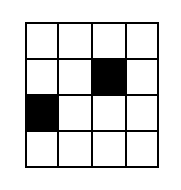
\includegraphics[scale=1.2]{figures/4by4.eps}
\caption{\label{fig:4by4}One active couple on a $4\times 4$ grid.}
\end{center}
\end{figure}
Then the signature of this image will be:
\begin{displaymath}
\begin{array}{ccccccc}
  &   &   & + & 0 & 0 & 0\\
0 & 1 & 0 & 0 & 0 & 0 & 0 \\
0 & 0 & 0 & 0 & 0 & 0 & 0 \\
0 & 0 & 0 & 0 & 0 & 0 & 0  
\end{array}
\end{displaymath}
All the translated views of this couple will give the same signature since the order of the similarity group of the active couple remains $5$.
\begin{figure}[!h]
\begin{center}

\includegraphics[scale=9.0]{figures/09by09.eps}
\caption{\label{fig:09by09}Multiple active couples on a $9\times 9$ grid.}
\end{center}
\end{figure}
Fig.~\ref{fig:09by09} shows a $9\times 9$ grid with $144$ similarity groups. All the active couples are counted to define the invariant signature. %Array~\ref{arr:01} 
The following array shows the translation invariant signature of Fig.~\ref{fig:09by09}:
\begin{displaymath}
\label{arr:01}
\begin{array}{ccccccccccccccccc}
  &   &   &   &   &   &   &   & + & 9 & 6 & 3 & 0 & 0 & 0 & 0 & 0\\
0 & 0 & 0 & 0 & 0 & 2 & 2 & 2 & 7 & 2 & 2 & 2 & 0 & 0 & 0 & 0 & 0\\
0 & 0 & 0 & 0 & 0 & 2 & 2 & 2 & 5 & 2 & 2 & 3 & 0 & 0 & 0 & 0 & 0\\
0 & 0 & 0 & 0 & 0 & 2 & 3 & 4 & 6 & 4 & 3 & 4 & 0 & 0 & 0 & 0 & 0\\
0 & 0 & 0 & 0 & 0 & 1 & 2 & 3 & 5 & 4 & 3 & 4 & 0 & 0 & 0 & 0 & 0\\
0 & 0 & 0 & 0 & 0 & 0 & 0 & 0 & 2 & 2 & 2 & 3 & 0 & 0 & 0 & 0 & 0\\
0 & 0 & 0 & 0 & 0 & 0 & 0 & 0 & 2 & 2 & 2 & 2 & 0 & 0 & 0 & 0 & 0\\
0 & 0 & 0 & 0 & 0 & 1 & 2 & 3 & 4 & 3 & 2 & 1 & 0 & 0 & 0 & 0 & 0\\
0 & 0 & 0 & 0 & 0 & 0 & 0 & 0 & 0 & 0 & 0 & 0 & 0 & 0 & 0 & 0 & 0\\
\end{array}
\end{displaymath}
%This signature is totally invariant to translation. This is quite obvious since each similarity group is translation invariant and the number of couples in a similarity group does not change by translation. 
In fact this array can be considered as a redefinition of an image in a new 3-D space having as axis the length, the slope and the number of couples. This 3-D space can be reduced to a 2-D space where the area covered by the slope and the length is represented by the similarity group order axis.
To find to which group a couple of points belongs, one should compare the length and slope of this couple to the length and slope of each similarity group.
Considering an $n \times n$ grid, we will have at most $2n(n-1)-1$ comparisons per couple and at most $(n^{2}!)/(2!(n^2-2)!)$ couples. Therefore, this comparison process for extracting the signature is rather slow.
For this reason we have formalized the access to the order number of the similarity groups by a simple function that eliminates the sequential comparison process.

Given two pixels $p$ and $q$ where the subscripts $r$ and $c$ refer to the row and the column, respectively, Algorithm \ref{alg:01} will find the similarity group number (SGN) $s$ of a couple.

\begin{pseudocode}[plain]{Get-SGN-T}{p, q, n}
 		s \GETS |q_c - p_c + (2n-1)(q_r-p_r)|\\
 \RETURN{s}
 \label{alg:01}
 \end{pseudocode}

This function yields the same number for all couples with equal slopes and equal lengths. Signature extraction is then performed by Algorithm~\ref{alg:est}, where $\mathcal{A}$ is the set of all active couples $(p, q)$.

\begin{pseudocode}[plain]{ExtractSignature-T}{\mathcal{A}, n}
	\LOCAL{t[2n(n-1)]}\\
	\FOR i \GETS 0 \TO 2n(n-1) \DO
		t[i] \GETS 0\\
	\FOREACH (p,q) \in \mathcal{A} \DO
		\BEGIN
		\LOCAL{s \GETS \CALL{Get-SGN-T}{p, q, n}}\\ 
		t[s] \GETS t[s]+1\\
		\END\\
 \RETURN{t}
 \label{alg:est}
 \end{pseudocode}

From here on, we can use the translation-invariant signature to define many other invariances, such as cylindrical or toric translation.

\subsection{Cylindrical Translation QIS}
Cylindrical translation (CT) invariance may seem useless in pattern recognition, but one of its possible applications will be shown below. 
Although the formal definition of a CT is quite difficult to establish, its  expression in terms of similarity groups is rather simple.
Fig.~\ref{fig:cyl} shows two possible positions of a couple of points in a CT. It can be seen that one couple of points in a CT can belong, at most, to two similarity groups of a simple translation.
\begin{figure}
\begin{center}
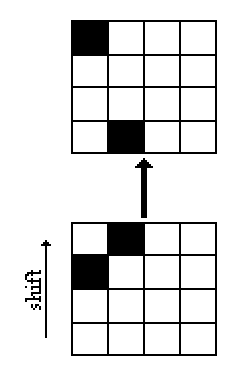
\includegraphics[scale=1.0, angle=-90]{figures/cyl.eps}
\caption{\label{fig:cyl}Cylindrical translation.}
\end{center}
\end{figure}
In this case the length of the couple and its slope are not unchanged by the CT anymore. If the two possible simple translation similarity groups are considered as the same similarity group for the CT, we can easily express the invariance to CT. QIS extraction remains exactly the same except for the SGN Algorithm. In this case, the additional SGN-CT function should find the second similarity group order number on the basis of the first number. When the couple is vertical, \ie, perpendicular to the translation direction, it will only define one similarity group.
Therefore, QIS extraction for a CT uses the same similarity groups as the simple translation, but the counting of combinations belonging to each similarity group is different. 

After applying Algorithm \ref{alg:01}, Algorithm~\ref{alg:ct} yields the correct order number of these groups.

\begin{pseudocode}[plain]{Get-SGN-CT}{s, n}
	\IF s < n 
\THEN t \GETS n-s
 	\ELSE
		t \GETS s - n [\textbf{signum}\{(s-n)\textbf{mod}(2n-1)-(n-1)\}] \\
 \RETURN{t}
 \label{alg:ct}
 \end{pseudocode}

%This function together with the function for calculating the original SGN will find the same numbers for all couples belonging to one of the two similarity groups. 
Signature extraction may be performed by Algorithm~\ref{alg:esct}, whereas the size of the signature will still be $2n(n-1)$. 

\begin{pseudocode}[plain]{ExtractSignature-CT}{\mathcal{A}, n}
	\LOCAL{t[2][2n(n-1)]}\\
	\FOR i \GETS 0 \TO 2 \DO
		\BEGIN
		\FOR j \GETS 0 \TO 2n(n-1) \DO
			t[i][j] \GETS 0\\
		\END\\
	\FOREACH (p,q) \in \mathcal{A} \DO
		\BEGIN
			\LOCAL{s[1] \GETS \CALL{Get-SGN-T}{p, q, n}}\\
			\LOCAL{s[2] \GETS \CALL{Get-SGN-CT}{s[1],n}}\\ 
			t[1][s[1]] \GETS t[1][s[1]]+1\\
			t[2][s[2]] \GETS t[2][s[2]]+1\\
		\END\\
 \RETURN{t}
 \label{alg:esct}
 \end{pseudocode}

\subsection{Toric Translation QIS}
Toric translation (TT) invariance can be used for regular texture recognition.
As for the CT case, we will use the simple translation similarity groups to define the TT signature.
The only thing to be added is the SGN-TT function and the number of similarity groups involved in a TT.
Fig.~\ref{fig:toric} shows four possible positions of a couple of points after a TT. Each couple of points in a TT can belong, at most, to four similarity groups of a simple translation.
\begin{figure}
\begin{center}
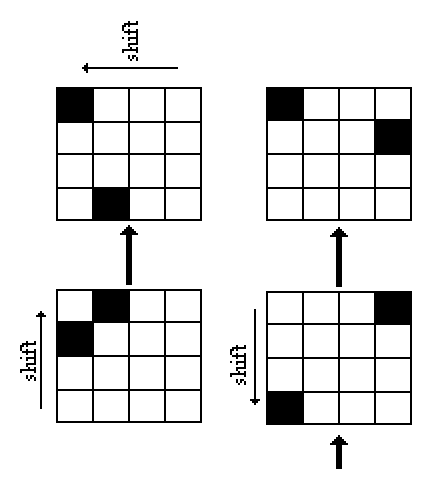
\includegraphics[scale=1.0, angle=-90]{figures/toric.eps}
\caption{\label{fig:toric}Toric translation.}
\end{center}
\end{figure}
In this case, QIS extraction follows the same reasoning as for CT.
The SGN function for TT QIS extraction is presented in algorithm~\ref{alg:tt}.

 \begin{pseudocode}[plain]{Get-SGN-TT}{s, n}
 	\IF s < n \THEN
		t \GETS s
	\ELSE
		t \GETS (2n-1)n-s\\
 \RETURN{t}
 \label{alg:tt}
\end{pseudocode}

This algorithm together with the previously described ones are used to determine the numbers corresponding to the four possible configurations. As a result, we can find the same numbers for all couples belonging to each of the four similarity groups. Signature extraction is then done as described by algorithm~\ref{alg:estt}. The size of the signature still remains $2n(n-1)$.

 \begin{pseudocode}[plain]{ExtractSignature-TT}{\mathcal{A}, n}
	\LOCAL{t[4][2n(n-1)]}\\
	\FOR i \GETS 0 \TO 4 \DO
		\BEGIN
		\FOR j \GETS 0 \TO 2n(n-1) \DO
			t[i][j] \GETS 0\\
		\END\\
	\FOREACH (p,q) \in \mathcal{A} \DO
		\BEGIN
			\LOCAL{s[1] \GETS \CALL{Get-SGN-T}{p, q, n}}\\ 
			\LOCAL{s[2] \GETS \CALL{Get-SGN-CT}{s[1], n}}\\ 
			\LOCAL{s[3] \GETS \CALL{Get-SGN-TT}{s[1], n}}\\ 
			\LOCAL{s[4] \GETS \CALL{Get-SGN-TT}{s[2], n}}\\ 			
			t[1][s[1]] \GETS t[1][s[1]]+1\\
			t[2][s[2]] \GETS t[2][s[2]]+1\\
			t[3][s[3]] \GETS t[3][s[3]]+1\\
			t[4][s[4]] \GETS t[4][s[4]]+1\\
		\END\\
 \RETURN{t}
 \label{alg:estt}
 \end{pseudocode}

\subsection{Symmetry QIS}
Symmetry invariance can also be coded by using the simple translation similarity groups and a new SGN function.
Fig.~\ref{fig:sym} shows two possible symmetric positions of a couple of points. One couple of points in a symmetry can belong, at most, to only two similarity groups of a simple translation.
\begin{figure}[h]
\begin{center}
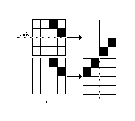
\includegraphics[scale=4.0, angle=0]{figures/symmetry.eps}
\caption{\label{fig:sym}Symmetry QIS.}
\end{center}
\end{figure}
Algorithm~\ref{alg:s} computes the two similarity groups involved in symmetry invariance.

 \begin{pseudocode}[plain]{Get-SGN-S}{s, n}
 	\IF s<n 
		\THEN
		 	t\GETS s
		\ELSE
			t\GETS s - 2 \{(s-n)\textbf{mod}(2n-1)-(n-1)\}\\
 \RETURN{t}
 \label{alg:s}
 \end{pseudocode}

\subsection{Size Invariant QIS}
In some cases, the size of the grid containing the reference pattern is not equal to the size of the grid containing the test pattern. QIS extraction can easily be adjusted to obtain invariance to grid size.
QIS of Fig.~\ref{fig:fov1} may be used to classify that of Fig.~\ref{fig:fov2}, or vice-versa.
\begin{figure}
\begin{center}
\subfigure[\label{fig:fov1}$16\times 16$.]{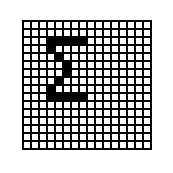
\includegraphics[scale=1.0]{figures/fovea1.eps}}
\subfigure[\label{fig:fov2}$32\times 32$.]{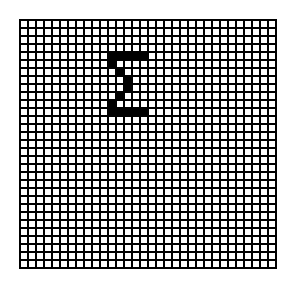
\includegraphics[scale=1.0]{figures/fovea2.eps}}
\caption{\label{fig:fov}Different size grids with same pattern.}
\end{center}
\end{figure}
The idea is to extract the QIS of the test image by using the size of the reference image.
Let $n \times n$ be the size of the test image and $m \times m$ be that of the reference image.

If $s$ is the order number of the similarity group of a couple on the $n \times n$ grid, then $s$ is found by one of the SGN functions defined earlier. The next step consists in finding the order number of the same group on the $m \times m$ grid. This is done by the following function:

 \begin{pseudocode}[plain]{Get-SGN-FS}{s, m, n}
 t \GETS s+2\lfloor \frac{s+n-1}{2n-1}|\rfloor (m-n) 	\\
 \RETURN{t}
 \label{alg:fs}
 \end{pseudocode}

QIS extraction is then performed by algorithm~\ref{alg:esfs1}, where {\scshape ExtractSignature} can be any of the signature extraction functions defined earlier.

\begin{pseudocode}[plain]{ExtractSignature-FS}{\mathcal{A}, m, n}
	\LOCAL{t[2m(m-1)]}\\
	\LOCAL{r[2n(n-1)]}\\
	r\GETS \CALL{ExtractSignature}{\mathcal{A},n}\\
	\FOR i \GETS 0 \TO 2m(m-1) \DO
		t \GETS 0\\
	\FOR i \GETS 0 \TO 2n(n-1) \DO
		\BEGIN
		\LOCAL{s \GETS \CALL{Get-SGN-FS}{i, m, n}}\\
		\IF s < 2m(m-1) \THEN
		t[s] \GETS r[i]\\
		\END\\
 \RETURN{t}
 \label{alg:esfs1}
 \end{pseudocode}

\subsection{Translation, Rotation and Scale QIS} \label{sec:trs}
Here we choose similar triangles as invariant primitives in the case of translation, rotation and scale (TRS) invariance. QIS extraction cannot be directly performed because counting the number of different triangles in an $n\times n$ grid is impossible. This problem seems to be open and, to the best of our knowledge, no formal solution exists.
Therefore we apply a simple and well-known log-polar space conversion to achieve TRS invariance. This conversion modifies a rotation to a cylindrical translation.
 
Let $P(\rho,\theta)$ be the polar coordinates of a point $p(x,y)$. In the polar imaginary space we will have $Z=\rho e^{\imath\theta}$.
If $P$ is rotated by $\alpha$ then $P_r(\rho,\theta+\alpha)$ and $Z_r=\rho e^{\imath(\theta+\alpha)}$.
If $P$ is scaled by a factor $k$ then $P_s(k\rho,\theta)$ and $Z_s=k\rho e^{\imath\theta}$.

Now let us consider the logarithm of $Z$:

$Z=\rho e^{\imath\theta} \implies \ln{Z} = \ln{\rho} + \imath\theta$.

Then 

$Z_r=\rho e^{\imath(\theta+\alpha)} \implies \ln{Z_r} = \ln{\rho}+\imath(\theta+\alpha)$ (translation along the $\imath$ axis);

$Z_s=k\rho e^{i\theta} \implies \ln{Z_s}=\ln{k}+\ln{\rho}+\imath\theta$ (translation along the $\ln{\rho}$ axis).

A translation in $(\ln\rho, \imath\theta)$ space defines a rotation and/or a scale change in $(x,y)$ space.
The only problem with this method is that the translation along the $\imath\theta$ axis is periodical, which implies that the translation along the $\imath\theta$ axis in the $(\ln\rho, \imath\theta)$ space is$\mod{360^\circ}$. 
Our QIS extraction for cylindrical translation is especially useful here.
The procedure to obtain the QIS for TRS is as follows:
\begin{enumerate}
\item Perform the space conversion to obtain the $log$-polar signature LPS; 
\item Extract the signature from the LPS matrix using Algorithm~\ref{alg:esct}.
\end{enumerate}

Fig.~\ref{fig:lnpolar} shows three examples of different images transformed into $\log$-polar coordinates.
\begin{figure}
\begin{center}
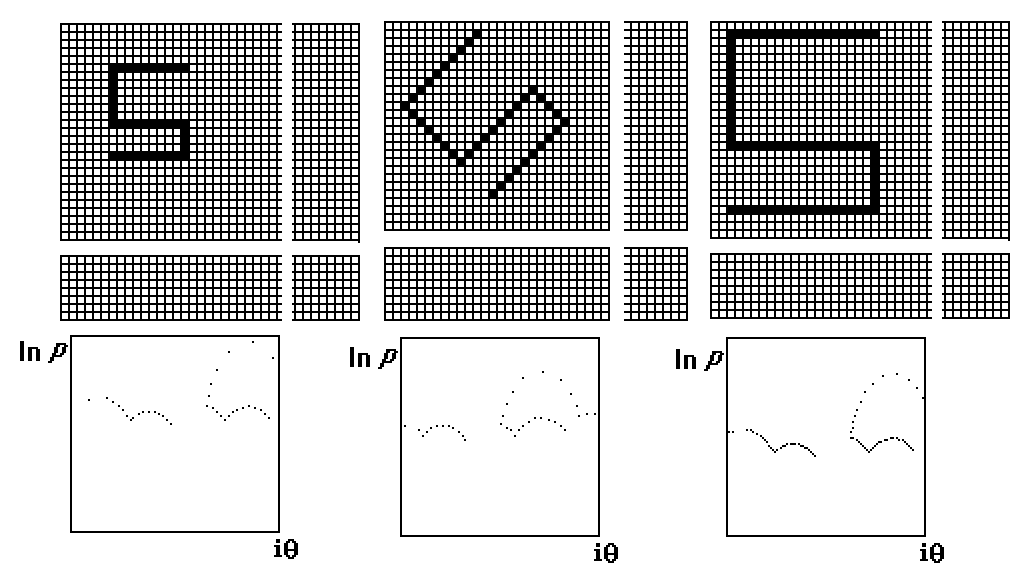
\includegraphics[scale=0.60]{figures/ln_polar.eps}
\caption{\label{fig:lnpolar}$\log$-polar transformation.}
\end{center}
\end{figure}
\subsection{Non-square grids}
So far we have discussed the case of square grids of $n\times n$. As to non-square grids, one quick solution would be to append zeros to the smallest dimension, which makes the matrix square and, then apply the already presented methods. However, we have developed a method that allows for direct processing of such grids. If we apply the space transformation presented in Section~\ref{sec:trs}, all we need is to do is redefine the translation invariant method for non-square grids, thus allowing the same reasoning applied to square grids to be applied to non-square ones. As the number of similarity groups in an $n \times m$ grid is $(n\times m-1) + (n-1)(m-1)$, most of the functions presented before do not need to be changed because they depend on the width of the image which is $n$. The only exception is the toric translation SGN which requires both the width $n$ and the height $m$ of the grid.

 \begin{pseudocode}[plain]{Get-SGN-TT-NS}{s, n, m}
 	\IF s < n \THEN
		t \GETS s
	\ELSE
		t \GETS (2n-1)m-s\\
 \RETURN{t}
 \label{alg:nonsq}
 \end{pseudocode}

The direct manipulation of the non-square matrices allows to set a different partitioning for each of the two axis (angle, logarithm) and get the best results according to the considered transformation.

Table~\ref{tab:examples} presents three examples of execution of the several discussed SGN functions to the transformations of Figs.~\ref{fig:ex1},~\ref{fig:ex2} and~\ref{fig:ex3}.
\begin{figure}
\begin{center}
\subfigure[\label{fig:ex1}]{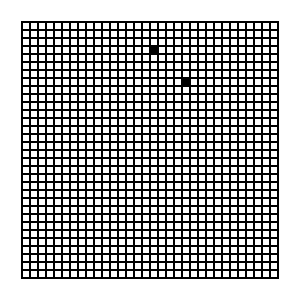
\includegraphics[scale=0.6]{figures/ex1.eps}}
\subfigure[\label{fig:ex2}]{\includegraphics[scale=0.6]{figures/ex2.eps}}
\subfigure[\label{fig:ex3}]{\includegraphics[scale=0.6]{figures/ex3.eps}}
\caption{\label{fig:examples}One active couple in each image.}
\end{center}
\end{figure}
\begin{table}[!ht]
\begin{center}
\begin{tabular}{c|cccccc}
\Hline
\bf Figure  & \multicolumn{2}{c}{\bf\ref{fig:ex1}} & \multicolumn{2}{c}{\bf\ref{fig:ex2}}& \multicolumn{2}{c}{\bf\ref{fig:ex3}}\\
\hline
\bf Pairs & \bf p & \bf q & \bf p & \bf q  & \bf p & \bf q \\
\Hline
\bf r&	4&	8&	22&	26&	1&	29\\
\bf c&	17&	21&	7&	11&	26&	22\\
\bf i&	113&	245&	679&	811&	801&	701\\
\hline
\bf T&	\multicolumn{2}{c}{132} & \multicolumn{2}{c}{132}& \multicolumn{2}{c}{1864}\\
\hline
\bf CT&	\multicolumn{2}{c}{[132, 1864]} & \multicolumn{2}{c}{[132, 1864]}& \multicolumn{2}{c}{[1864, 132]}\\
\hline
\multirow{2}{*}{\bf TT}&\multicolumn{2}{c}{[132, 1864,} & \multicolumn{2}{c}{[132, 1864,}& \multicolumn{2}{c}{[1864, 132,}\\
	&\multicolumn{2}{c}{1144, 924]}	&\multicolumn{2}{c}{1144, 924]}	&\multicolumn{2}{c}{1144, 924]}\\
\hline
\bf S&	\multicolumn{2}{c}{[132, 1120]} & \multicolumn{2}{c}{[132, 1120]}& \multicolumn{2}{c}{[1864, 156]}\\
\Hline
\end{tabular}
\end{center}
\caption {SGN of the transformations.}
\label{tab:examples}
\end{table}


\section{Adding more dimensions}
The QIS computation can be extended to more dimensions where most of the algorithms developed for the two-dimensional case can still be applied. Adding a new dimension is performed by applying two-dimensional SGN computations to the space that has one of the coordinates corresponding to an order of a group of the less-dimensional problem and the second coordinate corresponding to the added dimension.  
\begin{figure}[h]
\begin{center}
\includegraphics[scale=1.3]{figures/3dgrid1.eps}
\caption{\label{fig:3dgrid1} Calculation of a similarity group number for an active couple in $2\times 3 \times 3$ grid. First a similarity group number is extracted from $2 \times 3$ subspace. This signature is then used to position the pixels on an $8 \times 3$ grid which is used to calculate the final SGN.}
\end{center}
\end{figure}

We note here that it is possible to have different pixels with the same indexes in a lower-dimensional space. %This requires consideration of the case when two pixels have the same indexes. 
This problem is solved by allowing the signature group number to be zero in the lower-dimensional space. As a result, the number of similarity groups for an $m\times n \times o$ grid is equal to the number of similarity groups for the $(p+1)\times o$ grid, where p is the size of the $m\times n$ group. 

Another issue is that, for a pair of points, the ordering of them should be traced. This is done by preserving the sign of the similarity group number returned by the basic two-dimensional function. One can, at the end, get rid of this sign by taking the absolute value in the final dimension. 
Figs. \ref{fig:3dgrid1} and \ref{fig:3dgridsd} illustrate how the calculation of a similarity group is done in two particular situations.
\begin{figure}
\begin{center}
\includegraphics[scale=1.3]{figures/3dgridsd.eps}
\caption{\label{fig:3dgridsd} Calculation of a similarity group number of an active couple on a $2\times 3 \times 3$ grid in the case when the pixels coincide in the first two coordinates.}
\end{center}
\end{figure}
The modified two-dimensional SGN function is presented below:

\begin{pseudocode}[plain]{Get-SGN-2D}{p, q, n}
 		s \GETS q_c - p_c + (2n-1)(q_r-p_r)\\
 \RETURN{s}
 \label{alg:2d}
 \end{pseudocode}

The N-dimensional version of the function takes three vectors as parameters: $p$ and $q$ which contain the points' coordinates in all dimensions and $n$ which specifies the size of the grid in each dimension. \\

\begin{pseudocode}[plain]{Get-SGN-MD}{k, p, q, n}
	\LOCAL p', q'\\
	\LOCAL s' \GETS 1 \\
 	\IF k > 2 \THEN
   \BEGIN
		s' \GETS \CALL{Get-SGN-MD}{k-1, p, q ,n}\\
		 p'_r \GETS 1 \\
		 q'_r \GETS 1+|s'|\\
		\IF s' < 0 \THEN
      \BEGIN
         q'_c \GETS p[k]\\
         p'_c \GETS q[k]\\
		\END  
		\ELSE
      \BEGIN
		   q'_c \GETS q[k]\\
       	p'_c \GETS p[k]\\
      \END \\ 
	\END		\\
   \ELSE
	\BEGIN
		p'_r \GETS p[1]\\
		p'_c \GETS p[2]\\
		q'_r \GETS q[1]\\
		q'_c \GETS q[2]\\
      \END\\
s \GETS \mathbf{signum}(s')\CALL{Get-SGN-2D}{p',q',n[k]}\\
 \RETURN{s}
 \label{alg:md}
 \end{pseudocode}

\subsection{Recalculating the SGN in many dimensions}
Transformations such as shift and symmetry in a many-dimensional SGN require the specification of the coordinate in which the transformation occurs. In order to re-compute the order number of a group after such a transformation, when the original SGN is given, one needs to ``peel'' off the higher dimensions and obtain the order number of the group in the required dimension ``peeled off'' dimensions. Then signature extraction is applied using two-dimensional algorithms. Finally, the higher dimensionality is restored. 

In signature computation we take the pair ordering into account, as this may change due to the shift or symmetry transformations. This information is stored in the sign of the number returned by the recursive function. The final SGN will be obtained by taking the absolute value.

Below is the recursive algorithm which calculates the SGN after a shift operation in coordinate $i$. Here, $k$ is the number of dimensions of the space for which a signature $s$ was computed and $n$ is the vector holding the size of each dimension.

\begin{pseudocode}[plain]{Get-SGN-C-MD}{i, s, k, n}
	\IF i = k \THEN
   \BEGIN
		t \GETS \CALL{Get-SGN-CT}{s, n[k]}\\
		\IF t < n[k] \AND t > 0 \THEN
      t\GETS -t 
	\END		\\
   \ELSE
	\BEGIN
		\LOCAL s' \GETS \lfloor \frac{s+n[k]-1}{2n[k]-1}\rfloor\\
		\LOCAL t' \GETS \CALL{Get-SGN-C-MD}{i, s', k-1, n}\\
		t \GETS s + (|t'|-s')(2n[k]-1) \\
		\IF t' < 0 \THEN
		t \GETS -\CALL{Get-SGN-S}{(t,n[k])}\\
	\END\\
\RETURN{t}
 \label{alg:cmd}
 \end{pseudocode}

\begin{figure}
\begin{center}
\includegraphics[scale=0.8]{figures/3dshiftcalcul.eps}
\caption{\label{fig:3dshiftcalcul} Recalculation of the SGN for a shift operation in the coordinate $i=2$. All possible similarity group numbers are shown in the matrices. The active number is indicated by a frame. The ``peel off' operation can be seen as taking the row number (starting from 0) of the signature position in the table. The ``add back'' is then performed by changing the row according to the lower dimensional signature, but keeping the column of the previous signature.}
\end{center}
\end{figure}
\begin{figure}
\begin{center}
\includegraphics[scale=0.8]{figures/3dshift2calcul.eps}
\caption{\label{fig:3dshift2calcul} Recalculation of the SGN for a shift operation in the coordinate $i=1$. Note that, after a shift recalculation, the SGN is the same but the orientation has changed, which is indicated by reversing the content of the frames. Consequently, an additional symmetry operation is performed in upper spaces. }
\end{center}
\end{figure}
We note that the algorithm also works for for a shift in coordinate $i=1$ (see Fig. \ref{fig:3dshift2calcul}), which, in the two-dimensional case, corresponds to function {\scshape Get-SGN-TT}.

A similar solution can be applied if we want to get the SGN in case of a symmetry transformation. Compared to the previous example, the only thing that changes is the function for recalculating the SGN for a 2-D transformation, which is symmetry in this case.

\begin{pseudocode}[plain]{Get-SGN-S-MD}{i, s, k, n}
	\IF i = k \THEN
   \BEGIN
		t \GETS \CALL{Get-SGN-S}{s, n[k]}\\
		\IF t < n[k] \AND t > 0 \THEN
      t\GETS -t 
	\END		\\
   \ELSE
	\BEGIN
		\LOCAL s' \GETS \lfloor \frac{s+n[k]-1}{2n[k]-1}\rfloor\\
		\LOCAL t' \GETS \CALL{Get-SGN-S-MD}{i, s', k-1, n}\\
		t \GETS s + (|t'|-s')(2n[k]-1) \\
		\IF t' < 0 \THEN
		t \GETS -\CALL{Get-SGN-S}{(t,n[k])}\\
	\END\\
\RETURN{t}
 \label{alg:smd}
 \end{pseudocode}

In a similar way, the grid size can be changed. We only need to provide an additional parameter which is the modified grid size $m$ for a given coordinate number $i$. This operation does not change the pixel ordering. Therefore, the pseudo-code that deals with the orientation consistency can be skipped.

\begin{pseudocode}[plain]{Get-SGN-FS-MD}{i, m, s, k, n}
	\IF i = k \THEN
		t \GETS \CALL{Get-SGN-FS}{s, m, n[k]}\\
   \ELSE
	\BEGIN
		\LOCAL s' \GETS \lfloor \frac{s+n[k]-1}{2n[k]-1}\rfloor\\
		\LOCAL t' \GETS \CALL{Get-SGN-FS-MD}{i, m, s', k-1, n}\\
		t \GETS s + (|t'|-s')(2n[k]-1) \\
	\END\\
\RETURN{t}
 \label{alg:fsmd}
 \end{pseudocode}

The functions presented above may be considered as basic building blocks. By combining them, one can obtain a method to recompute a group's order number for more complicated operations. For example, if we want to get the SGN after shifts in both coordinates $i_1$ and $i_2$, then the result is obtained by:\\ {\scshape Get-SGN-C-MD }($i_2$,|{\scshape Get-SGN-C-MD }($i_1$,$s$,$k$,$n$)|,$k$,$n$).\\ This yields a correct SGN but may be computationally inefficient. Below we present an algorithm that recalculates the similarity group number for simultaneous shift operations in many dimensions.
Here $i$ is a boolean vector and for a given coordinate $k$, $i[k]$ indicates wether the shift in coordinate $k$ needs to be performed. Similar versions can be made for symmetry and grid-size change.

\begin{pseudocode}[plain]{Get-SGN-C-MD-V}{i, s, k, n}
	\LOCAL t \GETS 1 \\
	\IF k > 1 \THEN
	\BEGIN
		\LOCAL s' \GETS \lfloor \frac{s+n[k]-1}{2n[k]-1}\rfloor\\
		t' \GETS \CALL{Get-SGN-C-MD-V}{i, s', k-1, n}\\
		s \GETS s + (|t'|-s')(2n[k]-1) \\	
	\END\\	
	\IF i[k] \THEN
   \BEGIN
		s \GETS \CALL{Get-SGN-CT}{s, n[k]}\\
		\IF s < n[k] \AND s > 0 \THEN
      t'\GETS -t' 
	\END		\\
  \IF t' < 0 \THEN
		s \GETS -\CALL{Get-SGN-S}{(s,n[k])}\\
\RETURN{t}
 \label{alg:cmdv}
 \end{pseudocode}

%For a $k$ dimensional torus $2^k$ different configurations of a signature - with or without shifting - needs to be analyzed. However in practice one does not need to store and analyze all $2^k$ QIS numbers. It is enough to store one as the other may be obtained by applying functions given above. After evaluations of all of the variants one can choose to store only one minimal number.      


\begin{figure}
\begin{center}
\includegraphics[scale=0.75]{figures/3dsymmetry.eps}
\caption{\label{fig:3dsymmetry} Symmetry operations performed on one active couple. In the square braces note repeating similarity group numbers even if the positions of active pixels are different. After performing symmetry in all three dimensions the result has the SGN of an original image. In general, for a $n$-dimensional problem, one can have maximally $2^k-1$ unique similarity group numbers obtained by performing any combination of symmetry on an initial active couple. This number is equal to the number of diagonals of $n$-dimensional cube. For a shift operation one can obtain $2^k$ SGN numbers.}
\end{center}
\end{figure}



\section{Conclusions}
As demonstrated above, QIS is a very robust and time-saving method to extract a signature from a binary image and it also includes an extension to many dimensions. Nevertheless, it is difficult to formally demonstrate the uniqueness of QIS: a few totally symmetric patterns which produce the same QIS can be found. Of course, the uniqueness of QIS in case of asymmetrical patterns is intuitively evident. Even if the uniqueness of QIS can never be formally demonstrated, in practice the probability of finding the same QIS for two different patterns is nearly zero.

Another aspect to consider is related to the presence of noise. As QIS extraction uses couples of points, the introduction of one ``parasite'' pixel in an image, with a total of $n$ pixels, will introduce $n$ parasite couples. As the image is defined in terms of couples there will be a maximum of $n!/2!(n-1)!$ couples. Therefore, when the noise of an image is of the order of $1/n$ pixels, the number of couples will be $2/(n-1)$. It can be considered, then, that the perturbation has as factor of two. In spite of this theoretical disadvantage, QIS remains in practice much more robust in the presence of noise than other invariant recognition methods such as invariant moments \cite{Alt1962}. This is because QIS preserves the signature of the original image on a noisy grid. If we consider an image of $n$ pixels and one parasite pixel, the QIS extraction will show the QIS of the image incremented by $n$ parasite couples and the original signature is preserved although lightly incremented.
 

%% The Appendices part is started with the command \appendix;
%% appendix sections are then done as normal sections
%% \appendix

%% \section{}
%% \label{}

%% References
%%
%% Following citation commands can be used in the body text:
%% Usage of \cite is as follows:
%%   \cite{key}          ==>>  [#]
%%   \cite[chap. 2]{key} ==>>  [#, chap. 2]
%%   \citet{key}         ==>>  Author [#]

%% References with bibTeX database:

\bibliographystyle{natbib}
\bibliography{qis}

%% Authors are advised to submit their bibtex database files. They are
%% requested to list a bibtex style file in the manuscript if they do
%% not want to use model1a-num-names.bst.

%% References without bibTeX database:

% \begin{thebibliography}{00}

%% \bibitem must have the following form:
%%   \bibitem{key}...
%%

% \bibitem{}

% \end{thebibliography}


\end{document}

%%
%% End of file `elsarticle-template-1a-num.tex'.
